%Correct the file name.
%X: book number
%Y: part number
%ZZZ: page number in three digits. So page 3 would be 003.

\documentclass[12pt]{amsbook}

\usepackage{upgreek}
\usepackage{../HBSuerDemir}	% ------------------------
\footnote{usepackage{upgreek}}
\begin{document}

% ++++++++++++++++++++++++++++++++++++++
\hPage{b2p2/487}
% ++++++++++++++++++++++++++++++++++++++
\[y_c = c_1 u_1(x) + \dots + c_n u_n (x) \quad (obtained \quad by \quad P(\lambda)=0)\]
\\
\begin{enumerate}
    \item For
    \begin{align}
            \label{eq:b2p2_487_firstEquation}
             P(D)y &= f_i(x)
    \end{align}
    
    \noindent write the set
    \[S_i = \{\psi_1(x), \dots , \upvarphi_m(x)\}\]
    whose elements are $f_i(x) = \psi_1(x)$ and the functions appearing as terms in all derivatives (constants being ommited)
    \\
        \begin{enumerate}
            \item If none of $\upvarphi_i$ are contained in $\{u_1(x), \dots , u_n(x)\}$, then a particular solution $y_i$ is a linear combination of $\upvarphi_1 \dots , \upvarphi_m$:
            \[y_i = A_1\upvarphi_1(x) + \dots + A_m\upvarphi_m(x)\]
            and set this $y_i$ in (3) to obtain an identity yielding $m$ equations in the $m$ unknowns $A_1 , \dots , A_m$
            \\
            \item If some of $\upvarphi_i$ are conntained in $\{u_1 , \dots , u_n\}$, multiply each element of $S_i$ by the least power of $x$ to obtain a set $S_i'$ having no element in common with $\{u_1, \dots , u_n\}$. Then a linear combination of the elements in $S_i'$ is a particular solution whose coefficients are obtained as in a).
            \\
        \end{enumerate}
    \\
    \item Obtain in this manner all particular solutions $y_1 , \dots , y_k$ corresponding to $f_1(x) , \dots , f_k(x)$.\\
    Then the required PS will be
    \[y_p = y_1 + \dots + y_k.\]
\end{enumerate}
% =======================================================
\end{document}  

%==== templates ====

%==== environments ====

%\begin{figure}[htb]
%	\centering
%	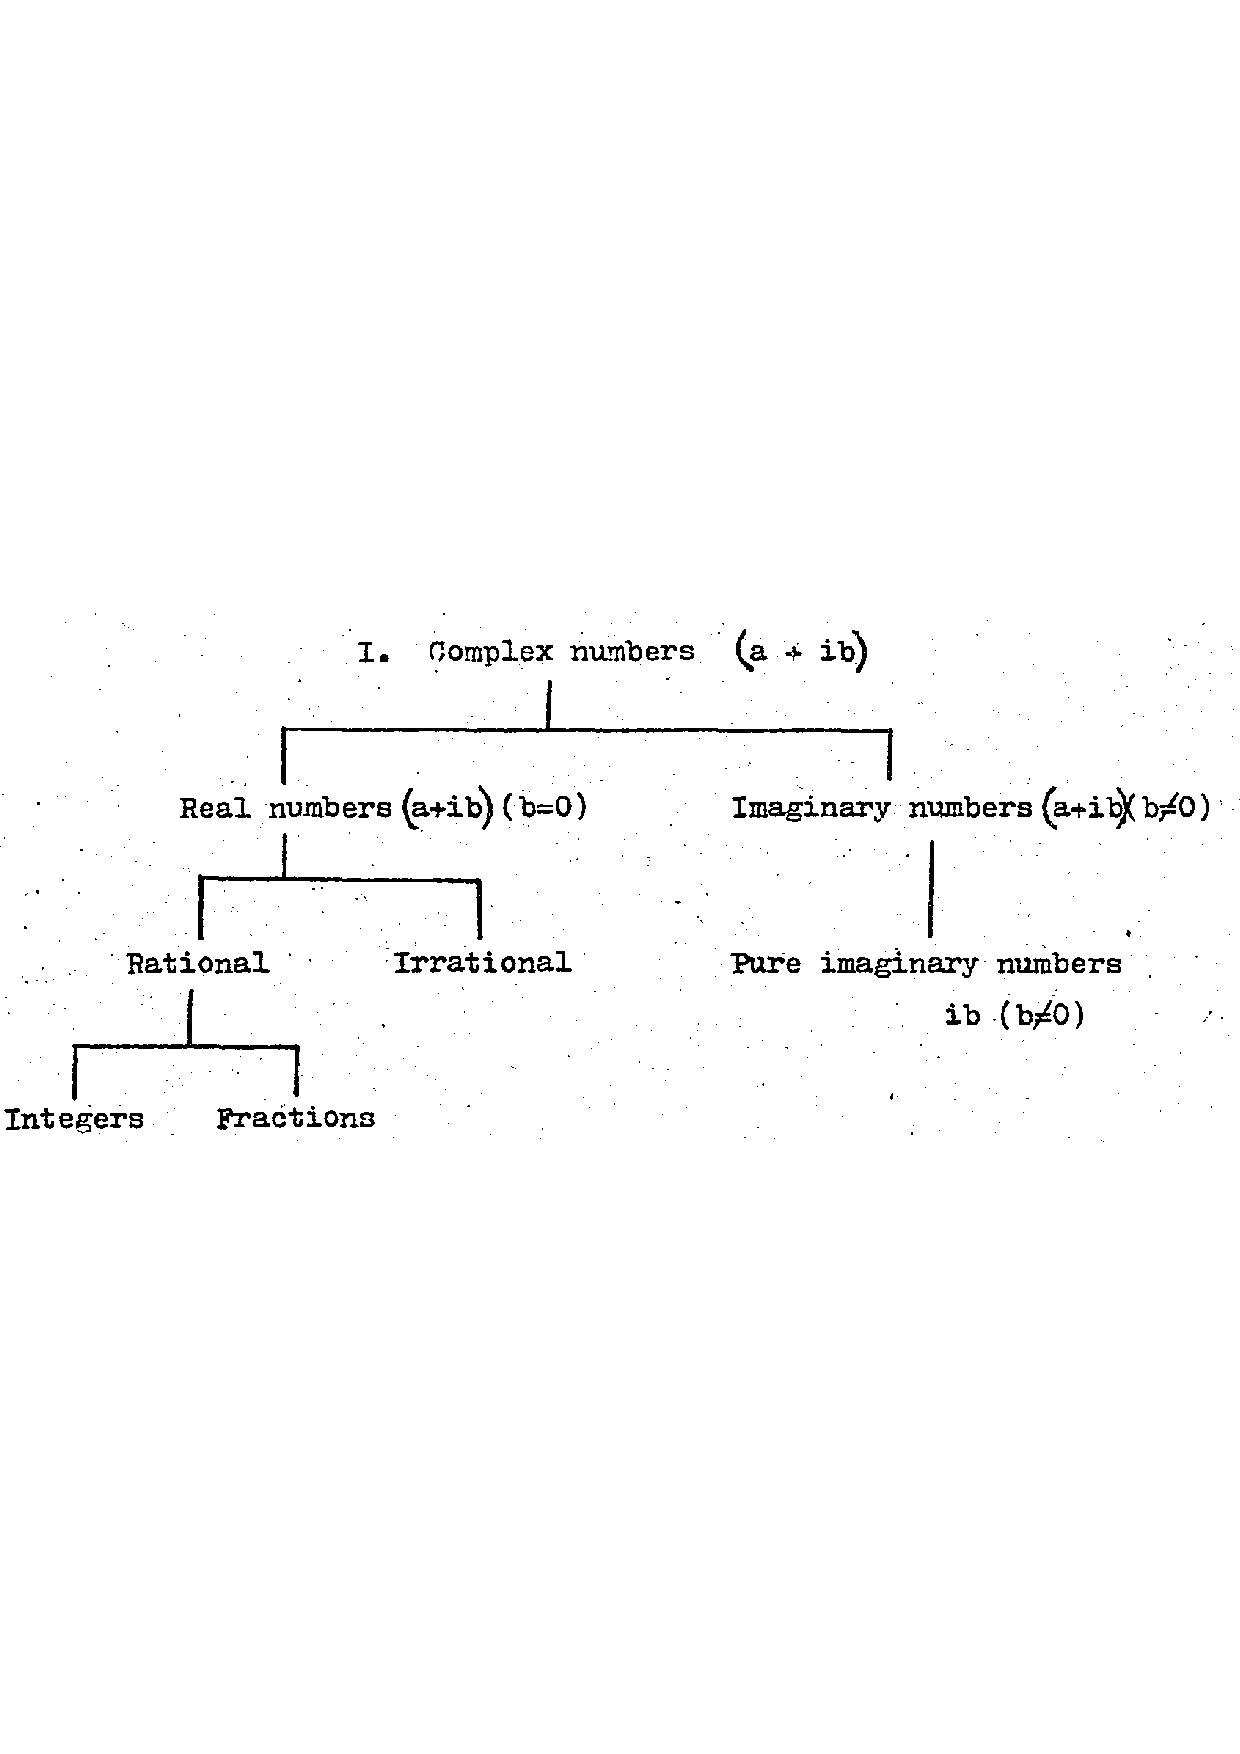
\includegraphics[width=0.9\textwidth]{images/SD-1-1p15A}
%	\caption{Classification of complex numbers}
%	\label{fig:classificationOfComplexNumbersA}
%\end{figure}

%\begin{center}
%\begin{tabular}{cc}
%\end{tabular}
%\end{center}

%\begin{exmp}
%\begin{hSolution}
%\end{hSolution}
%\end{exmp}

%\begin{hEnumerateAlpha}
%\end{hEnumerateAlpha}

%\begin{hEnumerateRoman}
%\end{hEnumerateRoman}

%$
%\begin{bmatrix}
%\end{bmatrix}
%$

%\frac{aaaa}{bbb}
%\frac{a_{n}}{b_{n}}
%\left( aaaa \right)
%\Longrightarrow

%\begin{multicols}{2}
%	bb
%\columnbreak
%	aa
%\end{multicols}
